\documentclass{article}

\usepackage[margin=4cm]{geometry}

\usepackage{tikz}
\usetikzlibrary{decorations.pathreplacing,decorations.markings}
\usetikzlibrary{arrows,positioning}
\usetikzlibrary{shapes.misc}

% style to apply some styles to each segment of a path
% This was the original style I went with for the edges, but it proved to
% look a little too busy
\tikzset{
  on each segment/.style={
    decorate,
    decoration={
      show path construction,
      moveto code={},
      lineto code={
        \path [#1]
        (\tikzinputsegmentfirst) -- (\tikzinputsegmentlast);
      },
      curveto code={
        \path [] (\tikzinputsegmentfirst)
        .. controls
        (\tikzinputsegmentsupporta) and (\tikzinputsegmentsupportb)
        ..
        (\tikzinputsegmentlast);
      },
      closepath code={
        \path [#1]
        (\tikzinputsegmentfirst) -- (\tikzinputsegmentlast);
      },
    },
  },
  % style to add an arrow in the middle of a path segment
  mid arrow/.style={
    postaction={
      decorate,decoration={
        markings,
        mark=at position .5 with {\arrow[#1]{stealth'}}
      }
    }
  }
}

\tikzset {
  % path style adds an arrow to each segment
  arr/.style = {
    draw = black,
    rounded corners = 2mm,
    postaction = {
      decorate,
      decoration = {
        markings,
        % Draw arrows manually to get them centered correctly, because this
        % isn't the default behavior for TIKZ
        mark=at position 0.5 with {
          \fill (2pt,0)--(-2pt,2.31pt)--(-2pt,-2.31pt)--cycle;
        }
%        mark=at position .5 with {\arrow[#1]{stealth'}}
      }
% Uncomment here (and comment out above) to enable per segment arrows
%      on each segment = {
%        mid arrow = black
%      }
    }
  },
  % path style with no arrows
  narr/.style = {
    draw = black,
    rounded corners = 2mm
  },
  % terminal symbol
  term/.style = {
    draw = black,
    rounded rectangle,
    inner sep = .2cm,
    font = \ttfamily
  },
  % non-terminal symbol
  nterm/.style = {
    draw = black,
    rectangle,
    inner sep = .2cm,
    font = \itshape
  },
  % support node
  entry/.style = {
    draw = black,
    circle,
    thick,
    minimum size = .2cm,
    inner sep = 0
  },
  node distance = 0.5cm
}

\title{Railroad Diagrams}
\date{}

\begin{document}

\maketitle

\section*{Module Block}

\begin{figure}[!h]
  \centering
  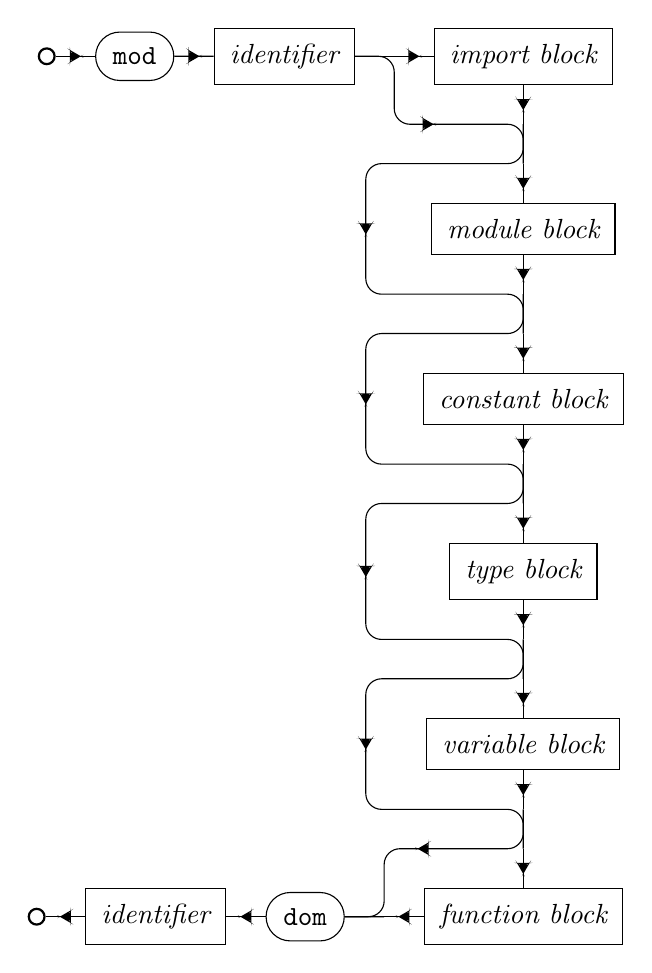
\begin{tikzpicture}
    \node[entry] (start) {};
    \node[term] (mod) [right=of start] {mod};
    \node[nterm] (mod name) [right=of mod] {identifier};

    \coordinate[right=of mod name] (name-imports);

    \node[nterm] (imports) [right=of name-imports] {import block};

    \coordinate[below=of imports] (imports-mods1);
    \coordinate[below=of imports-mods1] (imports-mods2);

    \node[nterm] (mods) [below=of imports-mods2] {module block};

    \coordinate[below=of mods] (mods-consts1);
    \coordinate[below=of mods-consts1] (mods-consts2);

    \node[nterm] (consts) [below=of mods-consts2] {constant block};

    \coordinate[below=of consts] (consts-types1);
    \coordinate[below=of consts-types1] (consts-types2);

    \node[nterm] (types) [below=of consts-types2] {type block};

    \coordinate[below=of types] (types-vars1);
    \coordinate[below=of types-vars1] (types-vars2);

    \node[nterm] (vars) [below=of types-vars2] {variable block};

    \coordinate[below=of vars] (vars-funcs1);
    \coordinate[below=of vars-funcs1] (vars-funcs2);

    \node[nterm] (funcs) [below=of vars-funcs2] {function block};

    \coordinate[left=of funcs] (funcs-dom);

    \node[term] (dom) [left=of funcs-dom] {dom};
    \node[nterm] (mod name end) [left=of dom] {identifier};
    \node[entry] (end) [left=of mod name end] {};

    % main line
    \draw[arr] (start) -- (mod);
    \draw[arr] (mod) -- (mod name);
    \draw[narr] (mod name) -- (name-imports);
    \draw[arr] (name-imports) -- (imports);

    \draw[arr] (imports) -- (imports-mods1);
    \draw[arr] (imports-mods2) -- (mods);

    \draw[arr] (mods) -- (mods-consts1);
    \draw[arr] (mods-consts2) -- (consts);

    \draw[arr] (consts) -- (consts-types1);
    \draw[arr] (consts-types2) -- (types);

    \draw[arr] (types) -- (types-vars1);
    \draw[arr] (types-vars2) -- (vars);

    \draw[arr] (vars) -- (vars-funcs1);
    \draw[arr] (vars-funcs2) -- (funcs);

    \draw[arr] (funcs) -- (funcs-dom);
    \draw[narr] (funcs-dom) -- (dom);

    \draw[arr] (dom) -- (mod name end);

    \draw[arr] (mod name end) -- (end);

    % side rail
    \draw[arr] (mod name)
      -- (name-imports)
      |- (imports-mods1)
      -- (imports-mods2);

    \draw[arr] (imports-mods1)
      -- (imports-mods2)
      -- ++(-2,0)
      |- (mods-consts1)
      -- (mods-consts2);

    \draw[arr] (mods-consts1)
      -- (mods-consts2)
      -- ++(-2,0)
      |- (consts-types1)
      -- (consts-types2);

    \draw[arr] (consts-types1)
      -- (consts-types2)
      -- ++(-2,0)
      |- (types-vars1)
      -- (types-vars2);

    \draw[arr] (types-vars1)
      -- (types-vars2)
      -- ++(-2,0)
      |- (vars-funcs1)
      -- (vars-funcs2);

    \draw[arr] (vars-funcs1)
      -- (vars-funcs2)
      -| (funcs-dom)
      -- (dom);
  \end{tikzpicture}
\end{figure}

\end{document}

